\subsubsection{Single Robot Dynamics}
In order to be able to comprehend the dynamics of the full system, with multiple robots and payload, we must first be able to understand the dynamics of a single freeflyer in a microgravity environment. We can derive the nonlinear dynamic equations of the system in with the Newton, referencing translation, and Euler, referencing rotation, equations. This can be seen in both \cite{roque2016space}, the main difference to this work is the use of quaternion for the representation of attitude, instead of the rotation matrix. Making the new equations be \ref{eq:Proposed approach: Motion Model: Nonlinear dynamics}, written with relation to the robot Center of Mass (CoM), where p, is the position of the robot, v is the velocity, q is the quaternion that represents the attitude of the robot, and $\omega$ is the angular velocity of the robot, this for variables constitute the state vector of the system, x= [p, v, q, $\omega$]. The system parameters here are J $\in \mathbb{R}^{3x3}$ is the inertia matrix of the robot, and m the mass of the robot.

\begin{equation}
    \begin{cases}
        &\dot{p} = v \\
        &\dot{v} =\frac{1}{m_i} R(q)F \\
        &\dot{q} = \frac{1}{2}Q(q) \omega \\ 
        &\dot{\omega} = J^{-1} \left(M -\omega \times J\omega \right) 
    \end{cases}
    \label{eq:Proposed approach: Motion Model: Nonlinear dynamics}
\end{equation}

The matrix R is the right-hand rotation matrix that converts from body frame to inertial frame. And the Q(q) $\in \mathbb{R}^{4x3}$ is the quaternion matrix as defined in \ref{eq:Proposed approach: Motion Model: Q matrix}

\begin{equation}
    Q\left(q\right) = 
    \begin{bmatrix}
        q_w && -q_z && q_y \\
        q_z && q_w && -q_x \\
        -q_y && q_x && q_w \\
        -q_x && -q_y && -q_z
    \end{bmatrix}
    \label{eq:Proposed approach: Motion Model: Q matrix}
\end{equation}

The vector M $\in \mathbb{R}^{3}$ is the torque applied in the robot, and F $\in \mathbb{R}^3$ is the force being applied. We can relate these to the system actuators according to \ref{eq:Proposed approach: Motion Model: Actuators}, where A is a matrix that converts from actuators space to torque and force space, and u in the actuation input vector of the system, meaning $u = \left[u_{1} \dots  u_{n} \right]^{T}$, where n is the number of actuators in the system and $u_{i}$ is the input of the i-th actuator. 

\begin{equation}
    \begin{pmatrix}
        F \\
        M
    \end{pmatrix} = A u
    \label{eq:Proposed approach: Motion Model: Actuators}
\end{equation}

\subsubsection{Multiple Robot Dynamics}

The dynamics presented for a single robot are not valid for the full system, since the connection between bodies also need to be taken into consideration, we can look at figure \ref{fig:Proposed Approach: Motion Model: Multi Robot System} to see a scheme of the connection.

\begin{figure}[H]
    \centering
    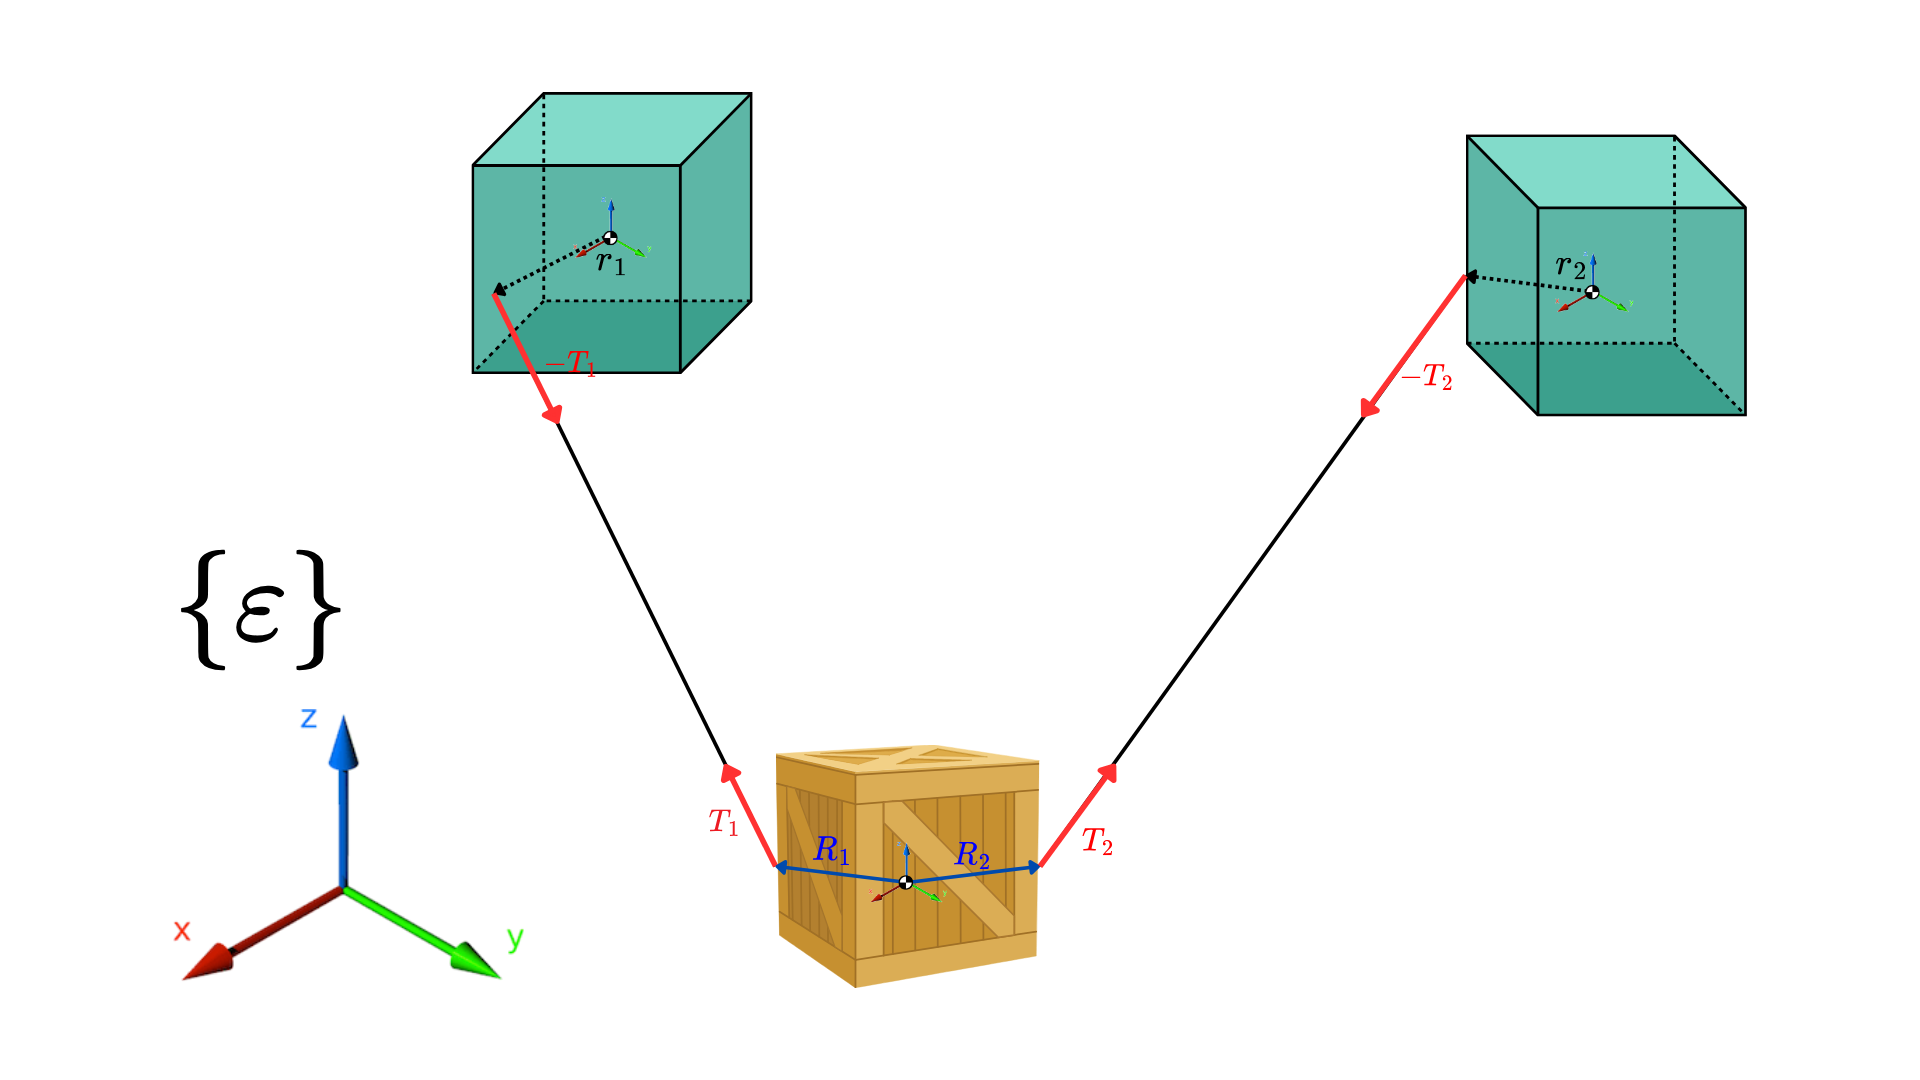
\includegraphics[width=0.7\textwidth]{Images/Propposed Aproach/multi body system.png}
    \caption{Multi Robot System}
    \label{fig:Proposed Approach: Motion Model: Multi Robot System}
\end{figure}

The dynamics of each robot in the formation will be as seen in equation \ref{eq:Proposed Approach:Motion Model: Multiple Robot Dynamics: Robot Dynamics}, where we can see the influence of the connection between the robot and the payload influence in the robot. The payload dynamics should also be considered,  we can see them in equation \ref{eq:Proposed Approach:Motion Model: Multiple Robot Dynamics: Payload Dynamics}, for both these equations the variables are defined in the following referential, $p_{i}$, $v_{i}$, $p_ {L}$, $v_{L}$, $T_{i}$ are in the inertial frame, $J_{i}$, $\omega_{i}$, $M_i$, $F_i$, $r_i$ are defined in the body frame of the i-th robot, and $J_{L}$, $\omega_{L}$, $q_L$ are defined in body frame of the payload. The matrices $R(q_{i})$ transforms from the i-th robot body frame to the inertial frame $\varepsilon$. The matrices $R(q_{i})^T$ and $R(q_{L})^T$ apply the transformation from inertial frame to the body frame of either the robot or the payload. And $N$ in the number of robots in the system.


\begin{equation}
    \begin{cases}
        \dot{p}_i &= v_{i} \\
        \dot{v}_i &= \frac{1}{m_i}\left[R(q_i)F_i - T_i\right] \\
        \dot{q}_i &= \frac{1}{2}Q(q) \omega_i \\
        \dot{\omega}_i &=J^{-1}\left[M_i - \omega \times J \omega - r_i \times R(q_i)^T T_i\right]
    \end{cases}
    \label{eq:Proposed Approach:Motion Model: Multiple Robot Dynamics: Robot Dynamics}
\end{equation}

\begin {equation}
    \begin{cases}
        \dot {p}_{L} &= v_{i} \\
        \dot {v}_{L} &= \frac{1}{m_{i}} \sum_{i = 1}^{N} T_{i} \\
        \dot {q}_{L} &=  \frac{1}{2} Q(q) \omega_{L} \\
        \dot{\omega_{L}} &= J_{L}^{-1} (-\omega_{L} \times J_{L} \omega_{L} + \sum_{i = 1}^{N} R_{i} \times \left[R(q_{L})^T T_{i}\right])
    \end{cases}
    \label{eq:Proposed Approach:Motion Model: Multiple Robot Dynamics: Payload Dynamics}
\end{equation}

This equations are independent of the method used to connect the robot, the dynamics will be valid, using both a robotic arm, or a simpler method of using a rope to connect, the only detail ones should take into consideration from this is, if the adopted method of connection to the payload is to use a rope, then $T_i \geq 0$, since otherwise work will not be exerted in the system, this will need to be taken into consideration for the design of the controller.